\documentclass[11pt,oneside,letterpaper]{article}

% graphicx package, useful for including eps and pdf graphics
\usepackage{graphicx}
\DeclareGraphicsExtensions{.pdf,.png,.jpg}

% basic packages
\usepackage{color}
\usepackage{parskip}
\usepackage{float}

% text layout
\usepackage{geometry}
\geometry{textwidth=15cm} % 15.25cm for single-space, 16.25cm for double-space
\geometry{textheight=22cm} % 22cm for single-space, 22.5cm for double-space

% helps to keep figures from being orphaned on a page by themselves
\renewcommand{\topfraction}{0.85}
\renewcommand{\textfraction}{0.1}

% bold the 'Figure #' in the caption and separate it with a period
% Captions will be left justified
\usepackage[labelfont=bf,labelsep=period,font=small]{caption}

% review layout with double-spacing
%\usepackage{setspace}
%\doublespacing
%\captionsetup{labelfont=bf,labelsep=period,font=doublespacing}

% cite package, to clean up citations in the main text. Do not remove.
\usepackage{cite}
%\renewcommand\citeleft{(}
%\renewcommand\citeright{)}
%\renewcommand\citeform[1]{\textsl{#1}}

% Remove brackets from numbering in list of References
\renewcommand\refname{\large References}
\makeatletter
\renewcommand{\@biblabel}[1]{\quad#1.}
\makeatother

\usepackage{authblk}
\renewcommand\Authands{ \& }
\renewcommand\Authfont{\normalsize \bf}
\renewcommand\Affilfont{\small \normalfont}
\makeatletter
\renewcommand\AB@affilsepx{, \protect\Affilfont}
\makeatother

% notation
\usepackage{amsmath}
\usepackage{amssymb}

%%% TITLE %%%
\title{\vspace{1.0cm} \Large \bf
ncov-forecasting-fit (title TBD)
}

\author[1,2]{Eslam Abousamra*}
\author[1,3]{Marlin Figgins*}
\author[1,2,4]{Trevor Bedford}

\affil[1]{Vaccine and Infectious Disease Division, Fred Hutchinson Cancer Center, Seattle, WA, USA}
\affil[2]{Department of Epidemiology, University of Washington, Seattle, WA, USA}
\affil[3]{Department of Applied Mathematics, University of Washington, Seattle, WA, USA}
\affil[4]{Howard Hughes Medical Institute, Seattle, WA, USA}


\date{}

\begin{document}

\maketitle

%%% ABSTRACT %%%
\begin{abstract}

Todo

\end{abstract}

%%% INTRODUCTION %%%
\section*{Introduction}

Modeling infectious diseases plays a key role in predicting growth of epidemics.
Understanding the trends and characteristics of emerging epidemics can guide public health officials to control their spread [Ding et al., 2021].
Epidemiologists face a multitude of challenges in order to provide accurate and timely predictions of disease spread.
With the increased availability of genomic sequencing, there has been efforts and potential in using sequences as a tool for investigating the genetic diversity, evolution, and transmission of epidemic-causing pathogens [Gire SK et al., 2014, Zhou et al., 2020]. 
More recently, with the deluge of data from various sources, issues with data arise regarding quantity, near-real-time accessibility, and quality.
%Integration of these data sources 
Data collected from different geographical locations and time-points exhibit varying degrees of issues with missing data, submission delays, and back-filling of disease occurence especially with a larger geographical scale [Pascal Crépey et al., 2022].
%preforming real-time analysis 
Thus, the quantities and the availability of genomic sequencing data differ depending on the date of observation and forecasting in varying geographical regions being studied.
This variability in sequences availability can have a significant impact on the accuracy and reliability of forecasting efforts using mathematical models [Suchard et al., 2018].
Furthermore, different modeling approaches may have varying levels of sensitivity to imperfections or limitations in the data.
Even when data is complete and accurate, the chosen model may not be suitable for the problem being analyzed, resulting in inability to capture target trends [Gelman et al., 2013].
Thereby, it is essential to take these factors (data-wise and systematic) into account when using mathematical models to make predictions, as they can impact the accuracy and reliability of the model's output [Pascal Crépey et al., 2022].


Mathematical models elucidate disease processes and have been sought to assess the risk and framing the response to emerging pathogens. 
%not mechanisms% 
Representation of disease spread from genomic sequences can not only help us forecast disease occurrence and pathogen frequencies, but also uncover the inherent characteristics of emerging pathogens and compare potential mechanisms of spread and persistence in the population [Metcalf et al., 2019].
%mention importance of forecasting variant frequences and estimating growth advantage
In particular, forecasting variant frequencies allows us to understand the impact of mutation accumulation and viral diversity on the spread and competition of different variants in the population.. 
Furthermore, by estimating variants growth advantages allows us to draw inferences regarding a biological selective advantage of specific variants which could potentially result in increased transmissibility or immune evasion [Tegally H. et al., 2021]. 
The validity and reliability of these mathematical models are dependent on the quality and quantity of data used for the model [Tao, K et al., 2021].
With the emergence of novel pathogens, real-time data scarcity represent a real challenge to accurate forecasts and also nowcasts, i.e forecasting on a short-term scale, as it leads to 
increased uncertainty in identifying and forecasting epidemic trends [Metcalf et al., 2019].







%what we actually did (high level)


In our efforts to investigate how modelling approaches handle data issues, we developed a framework for evaluating model nowcast and forecast of real-time SARS-CoV-2 variant frequencies.
%what is interesting about the framework (key points) comparing various models > applicable to real-time surveillance
In order to investigate the effectiveness of these different modeling approaches in the context of infectious disease prediction, we implemented the framework utilizing SARS-CoV-2 variants genomic sequence data as a input data for model comparison and evaluation.
%Specifically, we focused on models of increasing complexity, which were fitted using the evofr (evolutionary forecasting) software package in Python. 
To assess the performance of these models, we used several metrics such as MAE, RMSE, and Sequence log likelihood to compare the predicted frequencies to a set of known true values (Smoothed raw frequency values of SARS-CoV-2 variants). %what is truth set (Smoothed raw_freq)
This allowed us to evaluate the accuracy and reliability of the models and to identify those that were most effective in predicting SARS-CoV-2 circulating variants trends.

%What explains our errors
%try to explain the persistent patterns in the errors
In our study, we aimed to investigate the persistent patterns of errors in the different models used for nowcasting and forecasting the emergence of SARS-CoV-2 variants. 
To do so, we examined a variety of variables that may contribute to the emergence of errors in these models. 
Our goal was to identify the most important variables that play a role in our ability to forecast variant frequencies.
Through this analysis, we hope to gain a deeper understanding of the factors that contribute to errors in nowcasting and forecasting, and ultimately contribute to the ongoing efforts to understand and improve the accuracy of these models.
%limits of their use-ability 





%framework

%used it to make predictions (nowcasts and forecasts)


%scoring system to rate model preforamnes






%Common Methods to forecast from sequences












%I use Google Scholar format for citation style with first author, year and first word of title, ala \cite{hadfield2018nextstrain}.

%%% METHODS %%%
\section*{Methods}

Todo



* How different models handle imperfect data

\textbf{MLR}

\textbf{GARW}

\textbf{FGA}

\textbf{Piantham}

\textbf{Naive}


These models were implemented using the evofr (evolutionary forecasting) software package in Python.




%ga

The estimation shown of growth advantages are calculated relative to the baseline Omicron 21L (BA.1) strain, providing a point of reference for competing growth advantages and how median values change over time. 


* Framework

In our efforts to investigate how modeling approaches handle data issues, we developed a novel framework for standardizing and accurately estimating real-time nowcast and forecast targets, and to facilitate comparisons of forecasting and nowcasting accuracy between various statistical models.
This framework utilizes live surveillance data to examine the empirical aspects of evolutionary forecasting by forecasting targets which includes viral pathogen frequencies, pathogen growth advantages, and incidence estimates. 
Additionally, the framework provides a statistical scoring rule system for evaluating the effectiveness of different modeling approaches.
The purpose of this study is to investigate the utility of this framework in the context of evolutionary forecasting and to improve our understanding of the factors that influence the accuracy of nowcast and forecast targets.


\paragraph{Evaluation Criteria}\

RMSE was calculated as

%Equation

MAE was calculated as

%Equation

Logliklihood was calculated as

%Equation

%How to replicate the different analyses
%Talking about what variables mean




\section*{Data and code accessibility}

Sequence data including date and location of collection as well as clade annotation was obtained via the Nextstrain-curated
dataset that pulls data from GISAID database. 



Derived data of sequence counts and case counts, along with all source code used to analyze
this data and produce figures is available via the GitHub repository https://github.com/blab/ncov-forecasting-fit





%%% RESULTS %%%
\section*{Results} 

%TALKING ABOUT PROCESS FIGURES

\paragraph{Live Forecasting Environment}\

Figures presented in 1A and 1B offers a visual representation of the live nowcasting environment, illustrating the significance of incorporating observational data in our forecasting models and the variations that exist among countries in terms of the utilization and impact of such data.
We utilized the GARW model within the framework to demonstrate the dynamics of the live-estimation environment for five different SARS-CoV-2 variants specifically Omicron 21K, 21L, 21A, 22B, 22C (Figure 1A).
%MF:Being specific about the model isn't necessary here and which model can be mentioned in the caption alone. If we're talking about what's going on in Figure 1, I would say that directly and cite it \ref{fig:Figure1}
Utilizing sequencing data for these variants, we conducted a comparative analysis of the availability of SARS-CoV-2 variants sequences in Japan and the United States as observed for different observation dates along the period of April 22nd to June 15th, 2022 (Figure~\ref{Example data and predictions for Japan and USA}.A).

Throughout the observation period, the United States had a higher average availability of SARS-CoV-2 sequences compared to Japan. 
Nonetheless, both country exhibit variability in sequence availability count for the same dates depending on observation dates. 


We then evaluated the model performance by analyzing the input sequence data available for Japan and the United States on specific observation dates.
We used this data to predict the frequencies of SARS-CoV-2 variants in these countries, and compared these predictions to 7-day smoothed frequencies of variant occurrence (Figure~\ref{Example data and predictions for Japan and USA}.B).
However, it was observed that the model predictions for Japan were more frequently misestimated compared to United States.



%MF: In general, we want to be a bit more direct. These are not just the data there are predictions here as well. Really this figure is about a "Live nowcasting environment".
%%% map %%%
\begin{figure}[H]
	\centering
	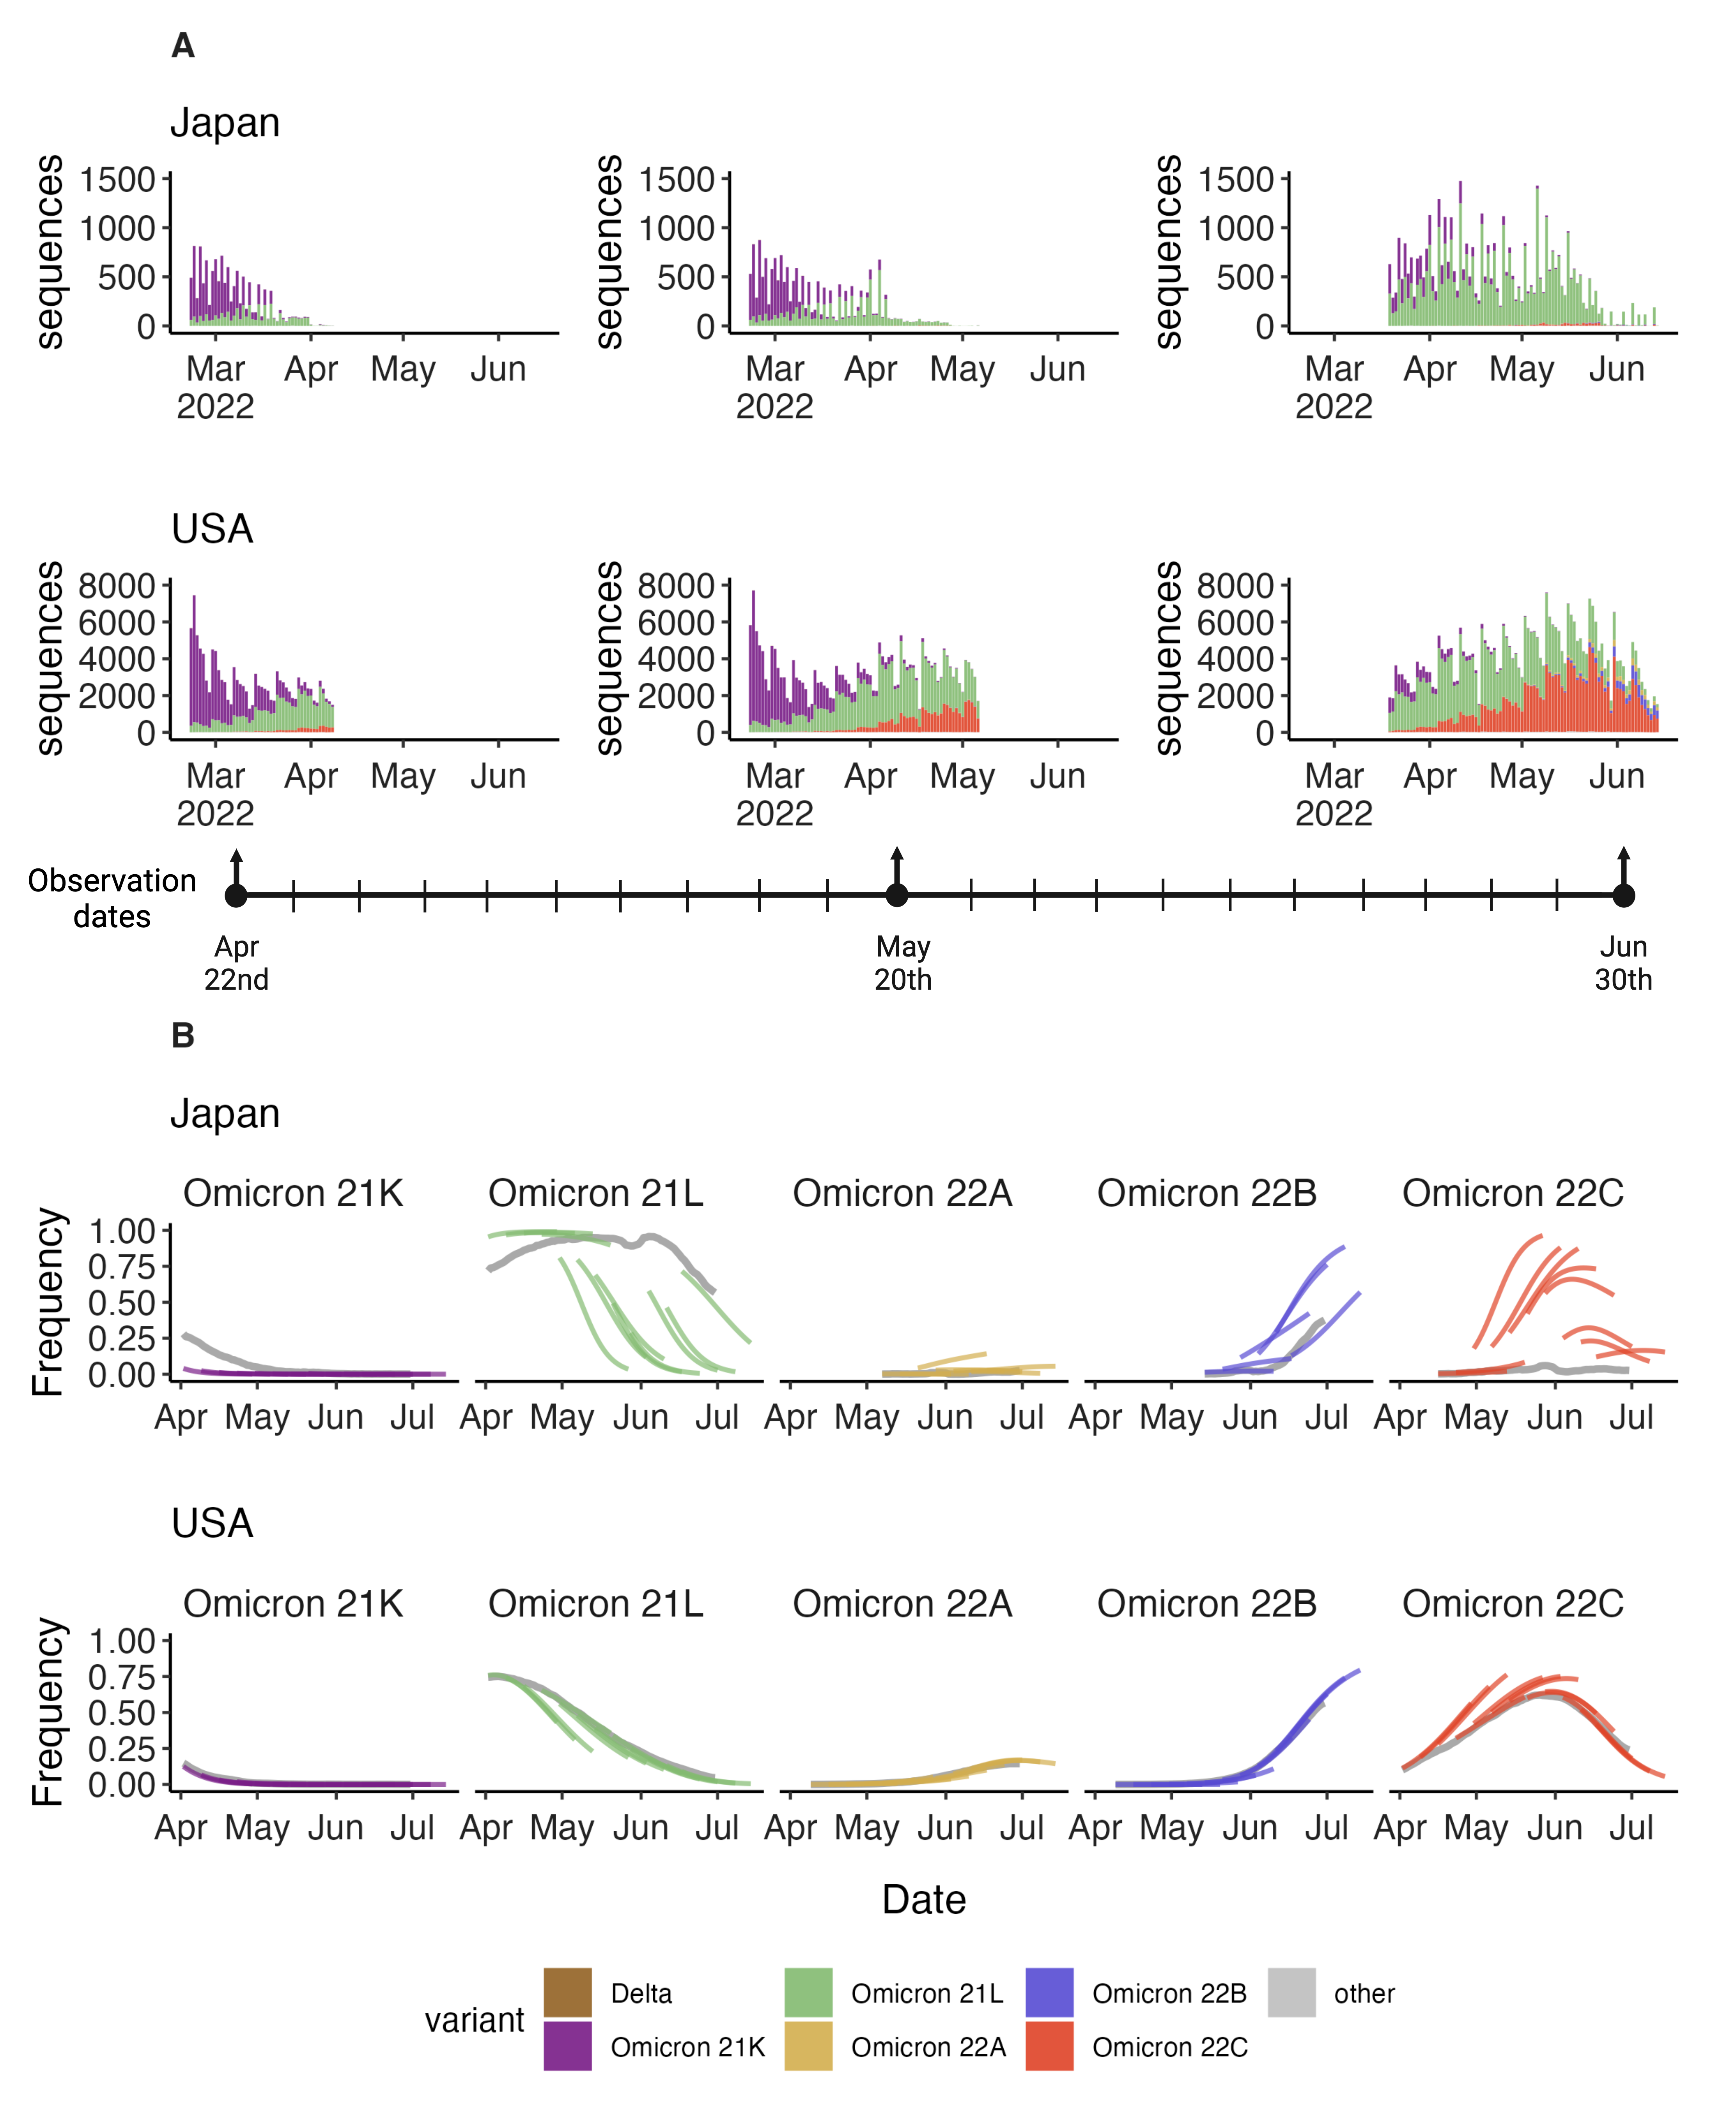
\includegraphics[width=0.8\textwidth=0.01]{figures/Figure1Final.png}
	\caption{\textbf{Example data and predictions for Japan and USA.}
  %MF: I would not say things like "Figure 1 represents". Just jump straight into the discription. 
  %MF: Example text might start with: Nowcasting variant frequencies is complicated by the continuous nature of the data submission process. (A) Variant sequence counts from Japan and United States are shown at 3 different observation dates. Notice ...
	Figure 1 represents a schematic of the dynamic estimation environment.
	Nowcasting variant frequencies is complicated by the continuous nature of the data submission process.
	(A) Variant sequence counts from Japan and United States are shown at 3 different observation dates.
	Notice varying sequence availability at different observation dates. 
	(B) Various frequency nowcasts which depends on the data are shown to vary predictions for different observation dates. 
	}
	\label{LiveNowcasts}
  %MF: Figure filenames and labels we typically want to describe what's in the figure itself since the order is usually subject to change.
\end{figure}


\paragraph{Model Error Comparison}\

We began our comparison by calculating the lag times (difference in days between the date of observation and the date of estimation) as a means of evaluating the performance of the models over time.
This approach provides a reference for understanding how the models perform as the lag time decreases from the forecast period to the nowcast period, where the lag time approaches zero (the date of estimation), specifically from [-30,30].
This enables us to evaluate the effectiveness of the models as we move closer to and further away from the date of observation.

We applied a total of five models for predicting the frequencies of SARS-CoV-2 variants in six countries spanning across different continents (Australia, Brazil, Japan, South Africa, United Kingdom, United States).
The first four models are GARW, FGA, MLR, and Piantham, which are evolutionary forecasting models... %write about whats common
We compare the above 4 models to a naive model to serve as a reference model for comparison.
It is a baseline model which uses simple assumptions to make predictions. 
The use of multiple models that ranges in complexity allows for a comprehensive evaluation of the performance and robustness of different forecasting methods.
In particular, the use of multiple models allows to examine if more complex models may be better at capturing epidemiological variant patterns. 

%Mention which models performed best in each lead (no need to mention numbers)
We used our predictions and used several metrics from the framework, specifically Mean Absolute Error (MAE), to assess the relative performance of the models for the six countries (Table~\ref{table1}).
The use of MAE as a metric allows us to quantitatively compare the predictions of different models and determine which model is most accurate in terms of predicting the frequencies of SARS-CoV-2 variants.
The model with the lowest mean MAE error for each country is highlighted as it indicates the best performance among all models (Table~\ref{table1}). 
The results showed that there was a range of values among the models for different leads.
In this study, the GARW model demonstrated best performance, on average, for -30 and 0 days from the date of estimation, when compared to the other models evaluated. 
Notably, for 30 days from the date of estimation, the MLR and GARW models both performed similarly well, with the MLR model exhibiting better performance in Australia, Brazil, and Japan, while the GARW model demonstrated better performance in South Africa, the United Kingdom, and the United States.
These findings indicate that the GARW model exhibited the best performance, as measured by mean absolute error (MAE), among the models evaluated, with the exception of the reference model (Naive).
In contrast, the Piantham model performed worst on average among the models tested.

\begin{figure}[H]
	\centering
	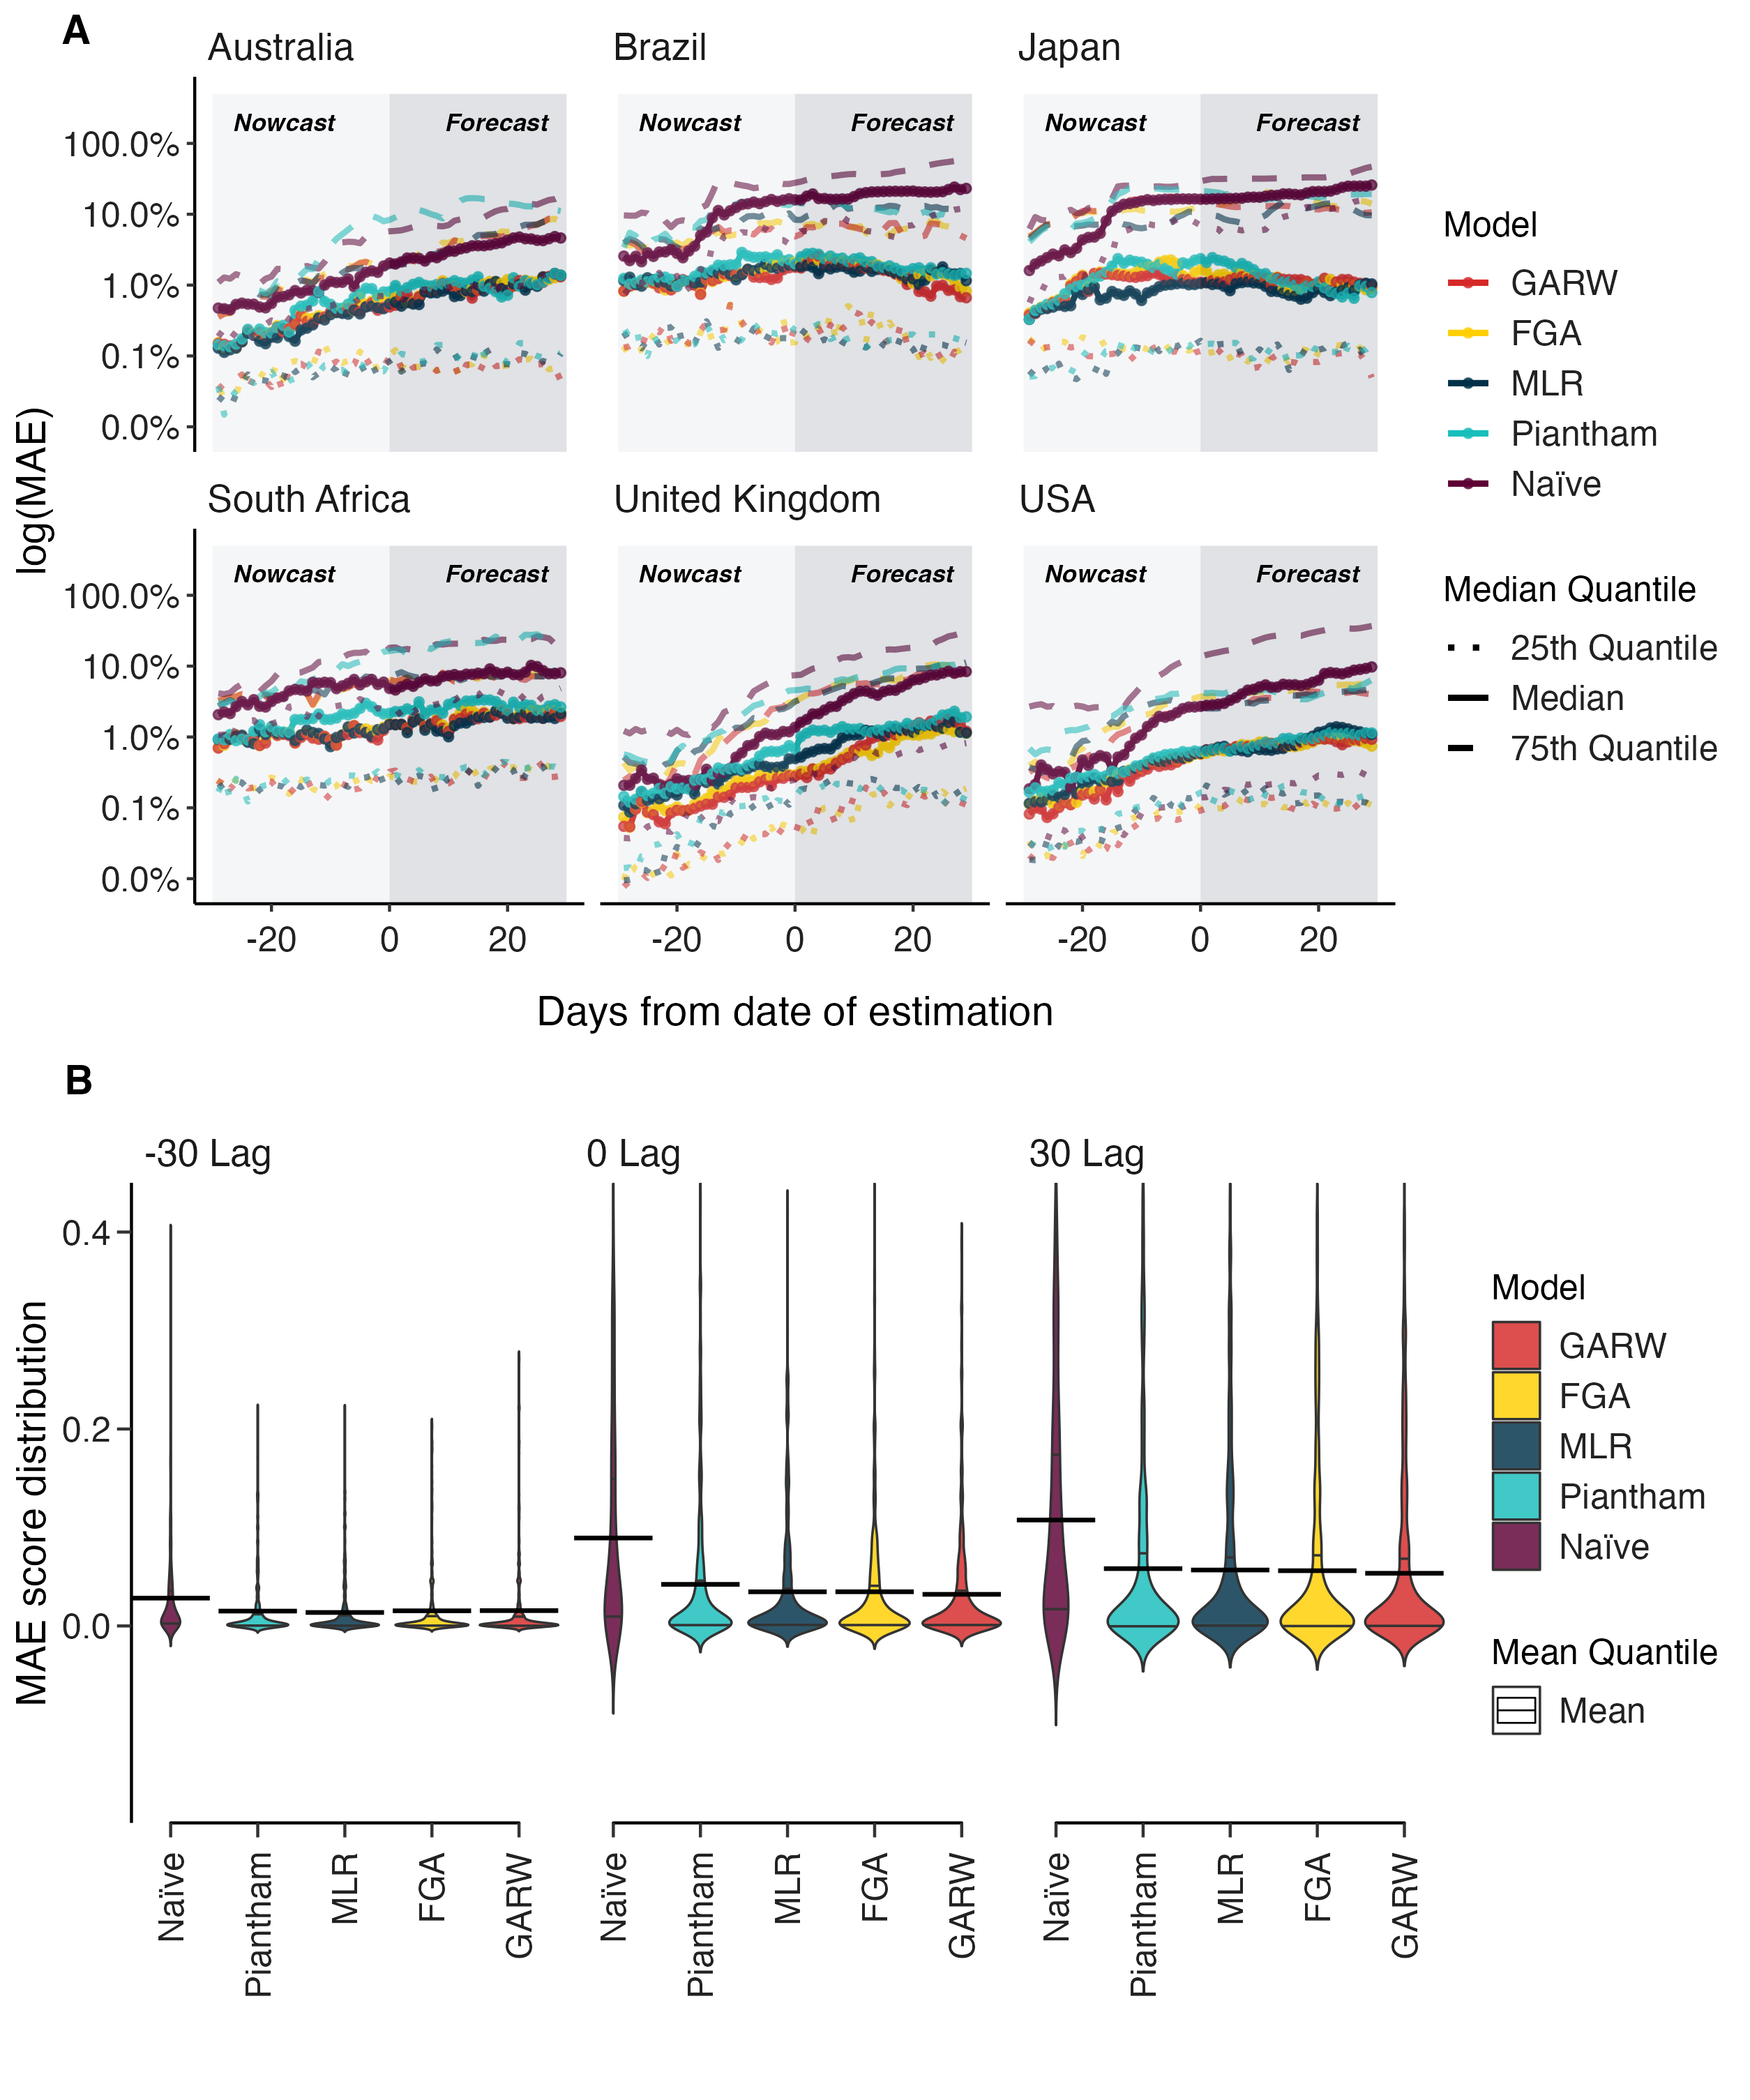
\includegraphics[width=0.8\textwidth]{figures/Figure2.png}
	\caption{\textbf{MAE estimates based on observation date.}
	Further legend here.
	}
	\label{Figure 2}
\end{figure}


Models were then compared side by side using error quantiles (25,50, and 75th percentile).
The majority of the models evaluated in this study exhibited median error values within the range of 0 to 10 percent of logarithm of mean absolute error (log(MAE)) (Figure~\ref{Figure 2}.A).
Furthermore,we compared the MAE score distribution between models for all countries (Figure~\ref{Figure 2}.B) .
As expected, the results of the analysis show an increase in MAE error for all models as lag or day from estimation increases. 
In other words, as forecasting step increases, the prediction accuracy for all models decreased.






\begin{table}[H]
	\centering
	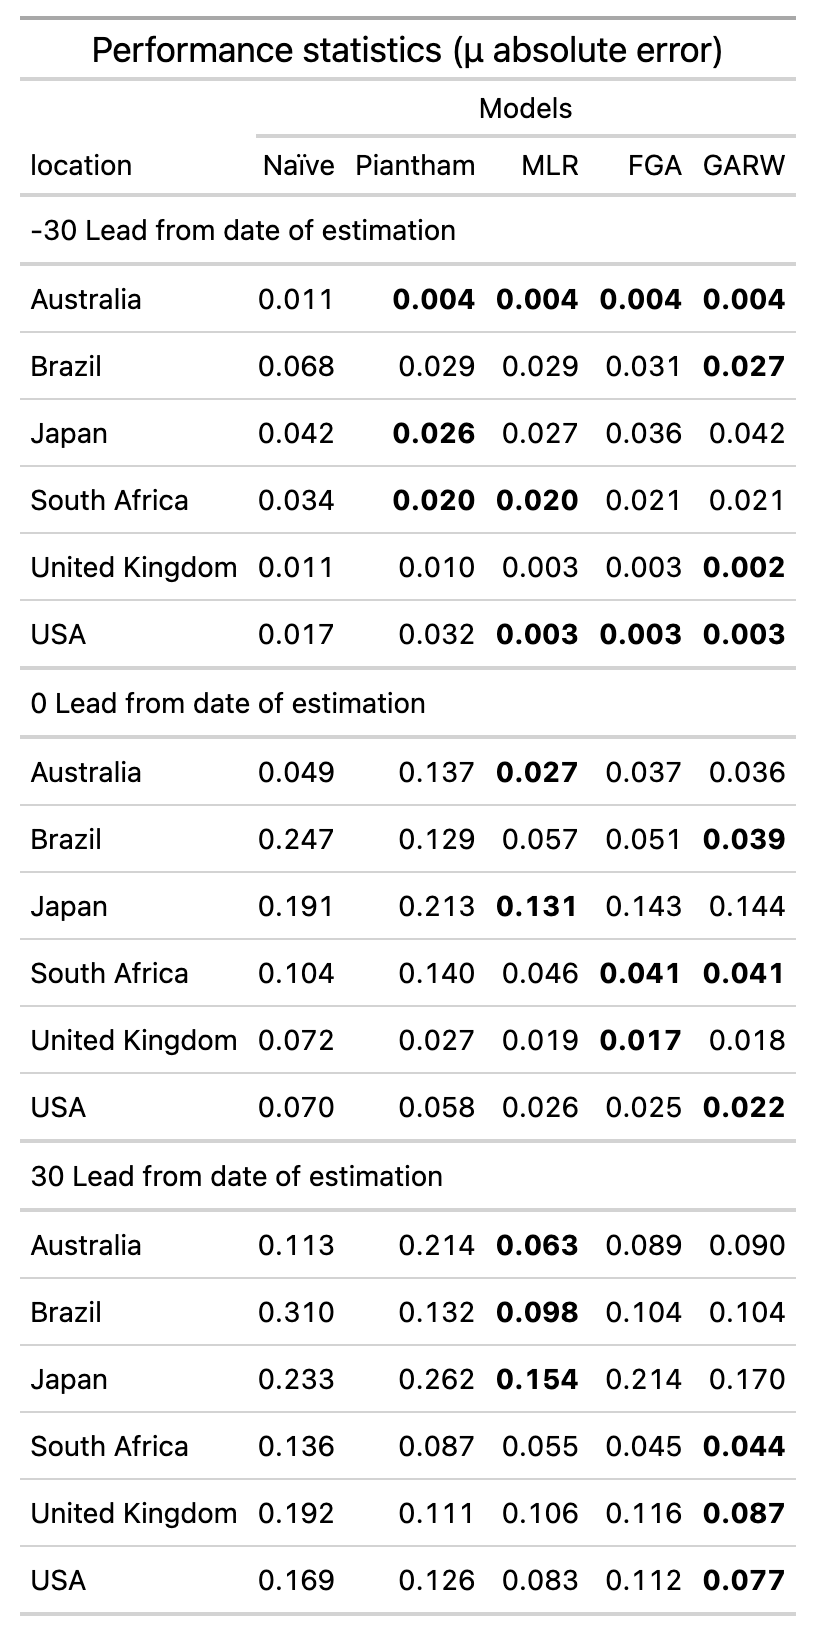
\includegraphics[width=0.6\textwidth]{figures/table1.png}
	\caption{\textbf{Mean Absolute Error}
	Further legend here.
	}
	\label{table1}
\end{table}




\paragraph{Comparison of Growth Advantages}\

Furthermore, In this study, we investigated the behavior of the growth advantage of different variants in various countries.

Using GARW, MLR, and Piantham models, we standardized the varying growth advantage by estimating the median Growth Advantage values as of that date, we were able to observe when and which variants stabilized in each country (Figure~\ref{Figure 3}). 
The results of the analysis revealed that the majority of countries displayed stabilization with regard to the Omicron 22A, B, and C variants, with the exception of Japan.
This discrepancy may be attributed to Japan's limited availability of sequence data or other imperfections in the data.
%they mostly stabilized except Japan % and why (motivated us to next step of analysis)


\begin{figure}[H]
	\centering
	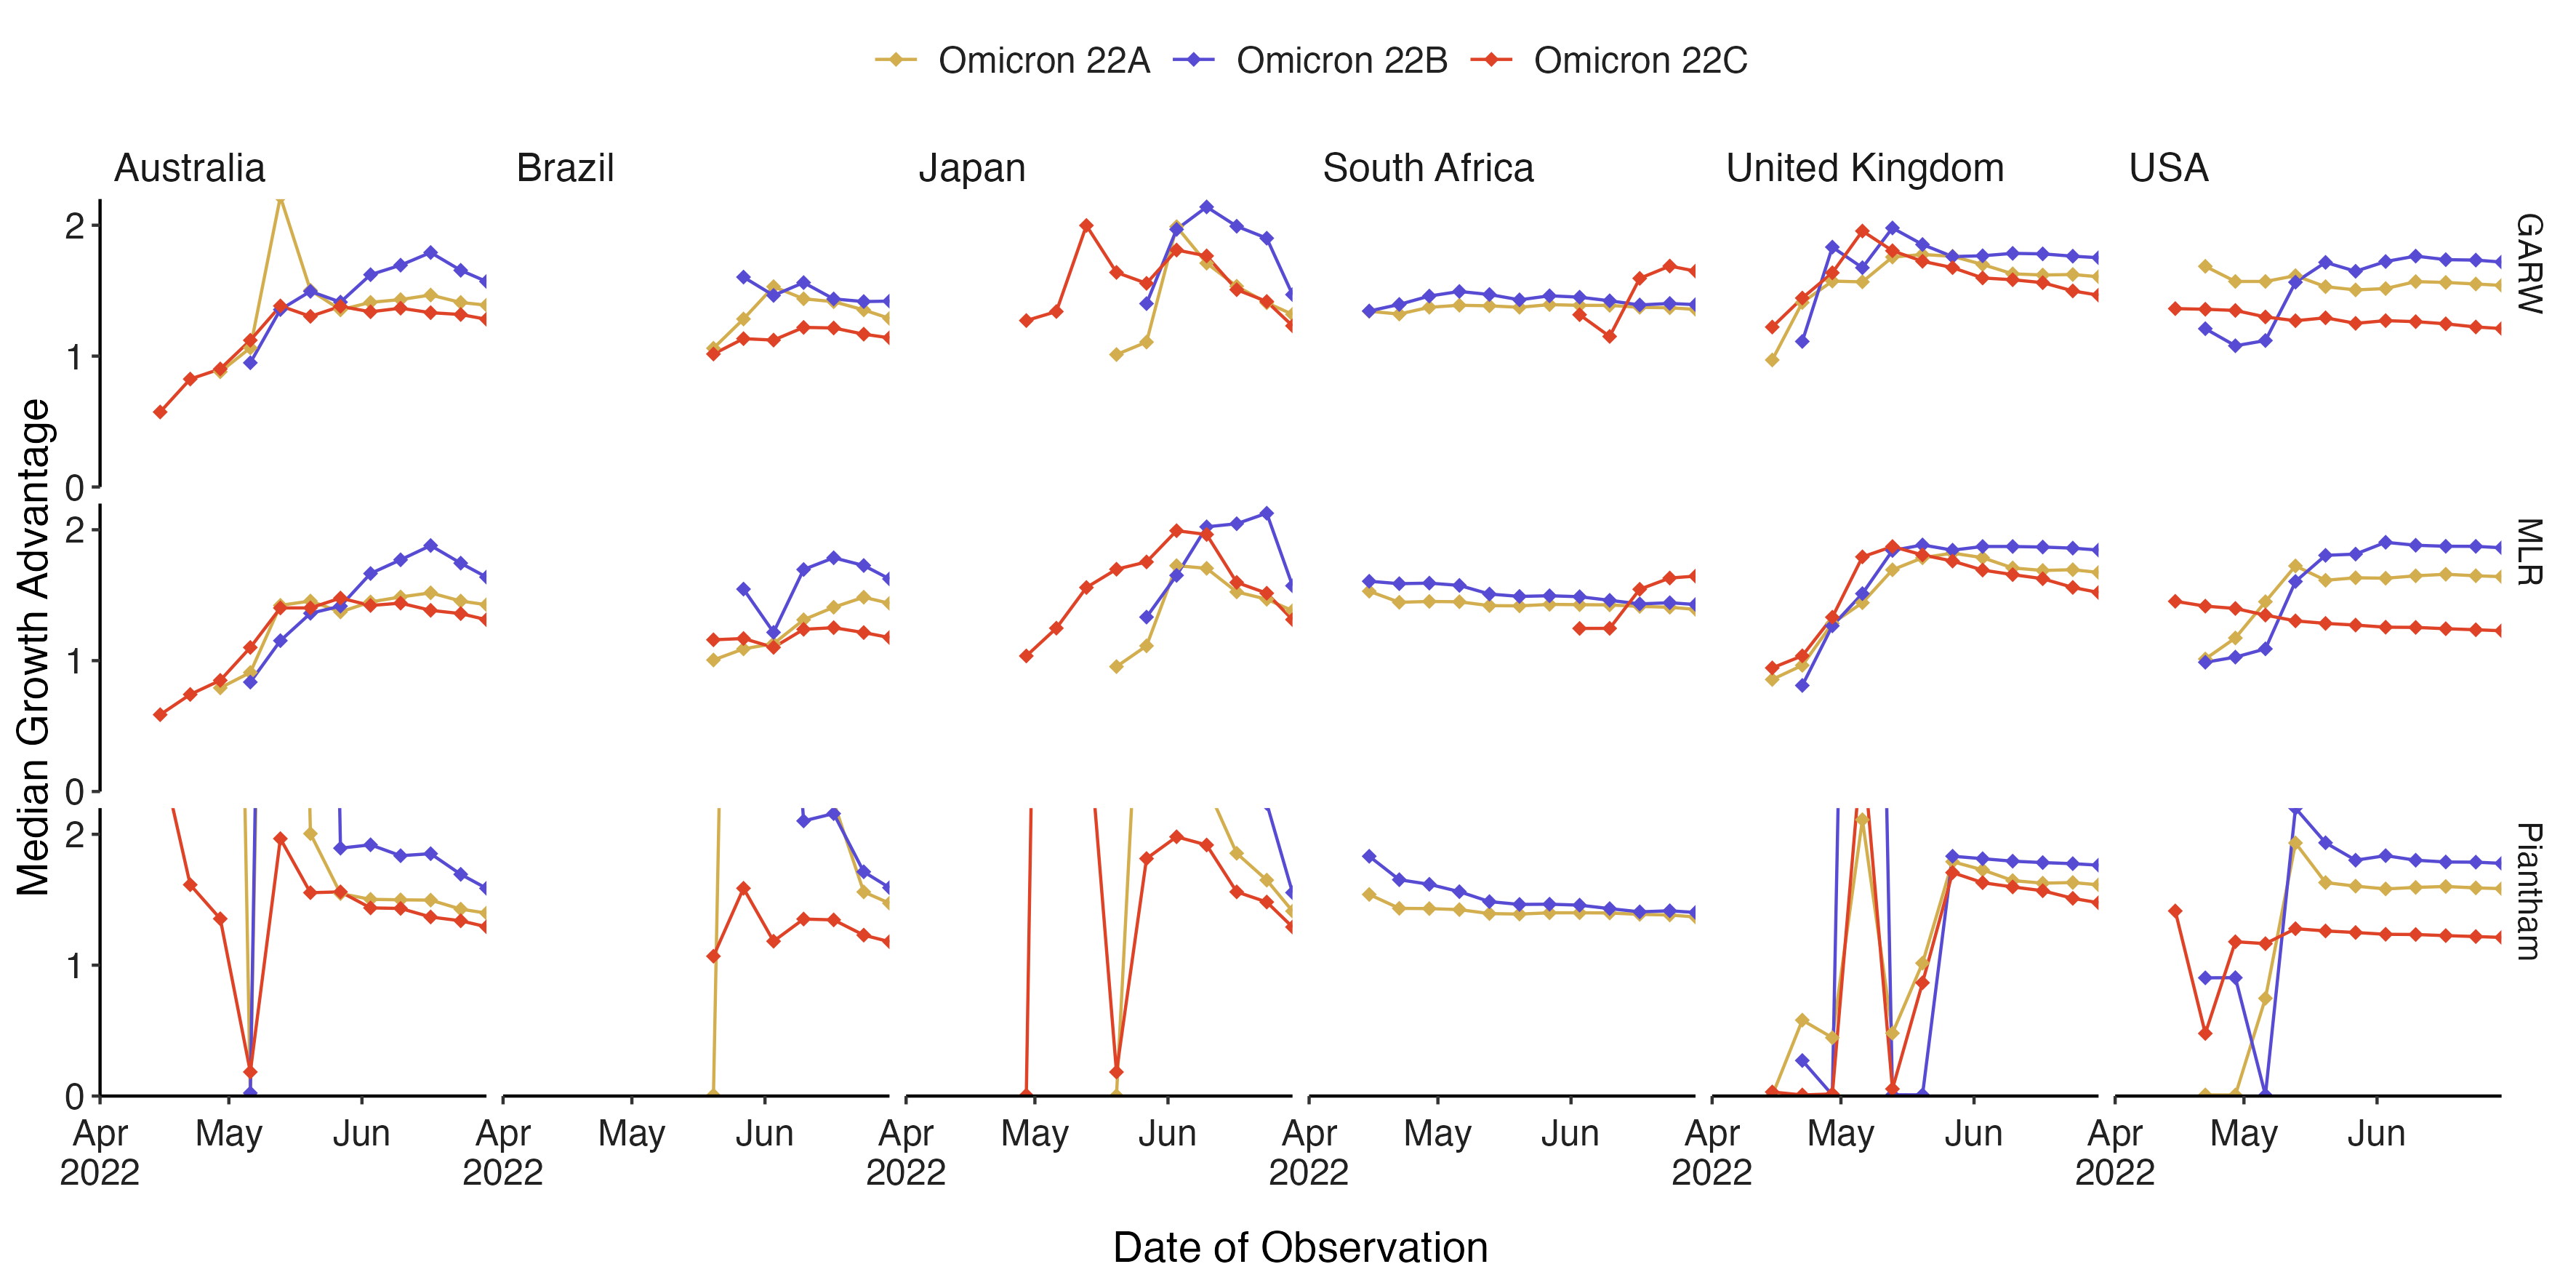
\includegraphics[width=1.1\textwidth]{figures/Figure3.png}
	\caption{\textbf{Growth Advantage of variants over time}
	Further legend here.
	}
	\label{Figure 3}
\end{figure}

\paragraph{Inferential Regression Model}\


\paragraph{Variation in frequency error}\

In order to investigate the variability among different countries and models and explain the emergence of error patterns in the forecasts, we employed a step-wise regression model to identify various variables that may contribute to errors in mean absolute error (MAE) of the models.
These variables were variants selective pressure, lead, sequence availability, fraction of sequences available within a week, median delay of data submission. 
Subsequently, a multivariate regression model was constructed to predict MAE errors, which was then fitted to SARS-CoV-2 variant data for all countries, as well as for each country individually.

\textbf{Model Specification}




maybe stepwise regression??

All countries model with logit transformation?

Model with interactions?

Mixture model?


Maybe just use correlations between the variables that we believe has an association?




log(MAE = xxxx)


\textbf{Model Performance}

R2 for each country (maybe make a table)
R2 for full model with all countries

Confidence intervals
prediction interval


%we built a linear model
% we picked these variables to predict the error
%identified which variables are of most importance
% 




%










%I put figures into a `/figures' directory and use semantic labeling ala (Figure~\ref{example_predictions}).










%%% DISCUSSION %%%
\section*{Discussion}

Todo

% Interpretation of the results

%Main findings

%Unexpected results

%Limitations

%Future research


%Conclusion







%%% REFERENCES %%%
\bibliographystyle{plos}
\bibliography{ncov-forecasting-fit}

\end{document}
